\section{lg\-Voice Class Reference}
\label{classlgVoice}\index{lgVoice@{lgVoice}}
a GUIDO voice with list(s) for events and tags  


{\tt \#include $<$lgvoice.h$>$}

Inheritance diagram for lg\-Voice::\begin{figure}[H]
\begin{center}
\leavevmode
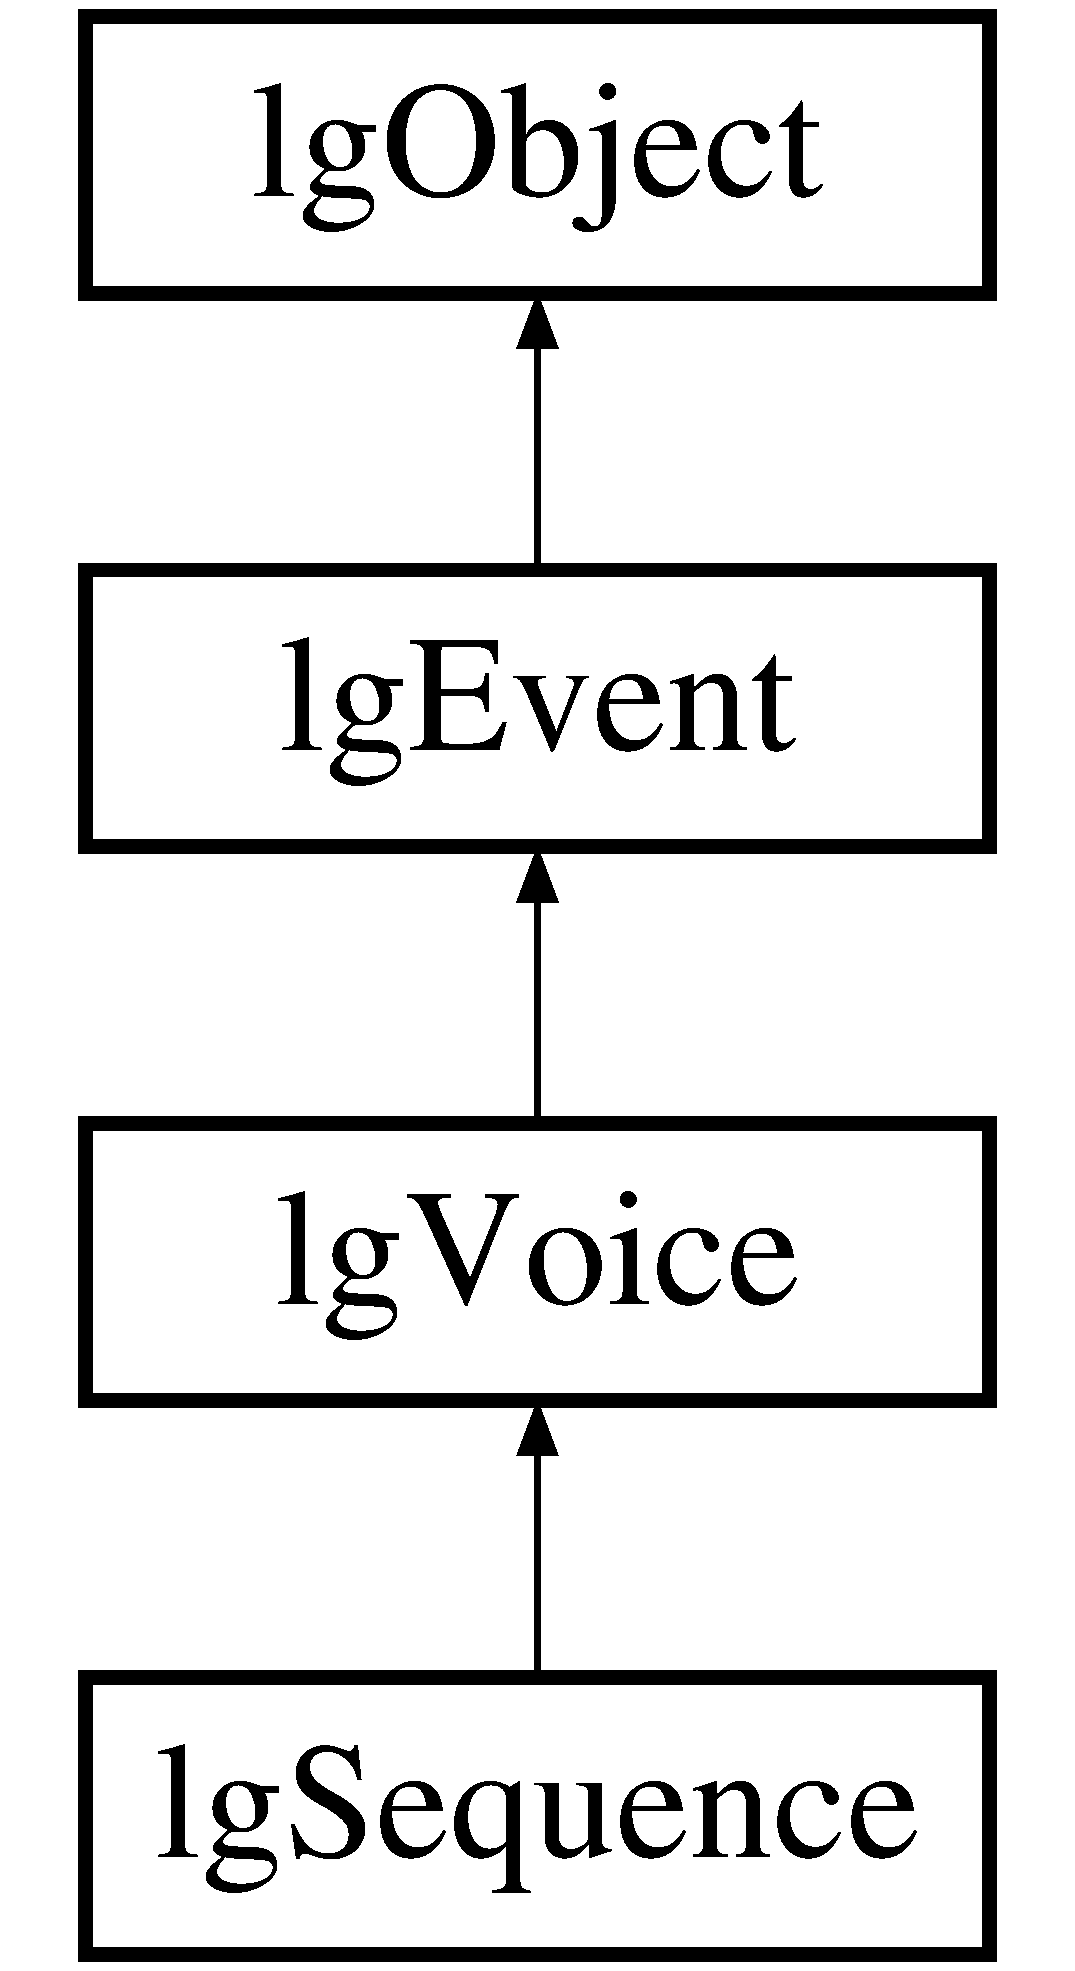
\includegraphics[height=4cm]{classlgVoice}
\end{center}
\end{figure}
\subsection*{Public Member Functions}
\begin{CompactItemize}
\item 
void {\bf replace\-Range\-Ptr} ({\bf lg\-Event} $\ast$old, {\bf lg\-Event} $\ast$new\-Ev)
\begin{CompactList}\small\item\em replace in all tags with prev\-Ev\-I==old\-Ev with new\-Ev \item\end{CompactList}\item 
virtual void {\bf set\-Next} ({\bf lg\-Voice} $\ast$seq)
\begin{CompactList}\small\item\em use also {\bf lg\-Chord::append\-Voice} as public function! \item\end{CompactList}\item 
virtual {\bf lg\-Tag} $\ast$ {\bf find\-Tag} (char $\ast$tag\-Name)
\begin{CompactList}\small\item\em search for a tag starting at beginning of the list \item\end{CompactList}\item 
virtual {\bf lg\-Tag} $\ast$ {\bf find\-Tag\-At} (const char $\ast$name, {\bf lg\-Duration} pos)
\item 
int {\bf delete\-Tag} ({\bf lg\-Tag} $\ast${\bf tag})
\begin{CompactList}\small\item\em return 1 if found \item\end{CompactList}\item 
int {\bf delete\-Event} ({\bf lg\-Event} $\ast$event)
\begin{CompactList}\small\item\em return 1 if found \item\end{CompactList}\item 
{\bf lg\-Voice} (long int pos\-Num, long int pos\-Denom)
\item 
virtual {\bf $\sim$lg\-Voice} (void)
\item 
void {\bf append\-Event} ({\bf lg\-Event} $\ast$ev)
\begin{CompactList}\small\item\em append at xx\-Tail \item\end{CompactList}\item 
void {\bf insert\-Tag} ({\bf lg\-Tag} $\ast${\bf tag})
\begin{CompactList}\small\item\em insert a tag in sorted taglist, if tag-$>$prev\-I == NULL -$>$ append at end of taglist! \item\end{CompactList}\item 
void {\bf close\-Tag} (long int no, {\bf lg\-Event} $\ast$ev, {\bf lg\-Factory} $\ast$factory)
\begin{CompactList}\small\item\em set end range of tag no \item\end{CompactList}\item 
string {\bf tags\-To\-String} ({\bf lg\-Event} $\ast$ev)
\begin{CompactList}\small\item\em write all tags between ev and ev-$>$next \item\end{CompactList}\item 
virtual {\bf lg\-Event} $\ast$ {\bf first\-Event} (void)
\begin{CompactList}\small\item\em this function doesn't look inside chords! \item\end{CompactList}\item 
virtual {\bf lg\-Event} $\ast$ {\bf next\-Event} ({\bf lg\-Event} $\ast$ev)
\begin{CompactList}\small\item\em this function doesn't look inside chords! \item\end{CompactList}\item 
virtual {\bf lg\-Note} $\ast$ {\bf first\-Note} (void)
\item 
virtual {\bf lg\-Note} $\ast$ {\bf next\-Note} ({\bf lg\-Event} $\ast$ev)
\item 
virtual long int {\bf c\-Notes} (void)
\begin{CompactList}\small\item\em return number of existing notes. Might be different to {\bf events}! \item\end{CompactList}\item 
virtual {\bf lg\-Tag} $\ast$ {\bf first\-Tag} (const char $\ast$n=NULL)
\begin{CompactList}\small\item\em get first tag with name == n \item\end{CompactList}\item 
virtual {\bf lg\-Tag} $\ast$ {\bf next\-Tag} ({\bf lg\-Tag} $\ast${\bf tag})
\item 
virtual char {\bf insert\-Event} ({\bf lg\-Event} $\ast$event)
\begin{CompactList}\small\item\em insert a event at event-$>$pos \item\end{CompactList}\item 
virtual string {\bf to\-String} ({\bf lg\-Voice} $\ast$calling\-Seq=NULL)
\item 
virtual void {\bf write} (FILE $\ast$out, {\bf lg\-Voice} $\ast$v=NULL)
\begin{CompactList}\small\item\em write to .gmn \item\end{CompactList}\item 
virtual lg\-Frac {\bf duration} (void)
\begin{CompactList}\small\item\em return duration of voice, events\-Tail must be uptodate! \item\end{CompactList}\item 
virtual {\bf lg\-Tag} $\ast$ {\bf find\-Tag} (long int id)
\begin{CompactList}\small\item\em search for tag in tag list and all chords \item\end{CompactList}\item 
virtual {\bf lg\-Event} $\ast$ {\bf find\-Event} ({\bf lg\-Duration} at\-Pos)
\begin{CompactList}\small\item\em search for event with event-$>$pos == at\-Pos, return NULL if not found \item\end{CompactList}\item 
{\bf lg\-Event} $\ast$ {\bf event\-Hold\-At} ({\bf lg\-Duration} pos)
\begin{CompactList}\small\item\em check if an event is holding at pos \item\end{CompactList}\item 
{\bf lg\-Event} $\ast$ {\bf latest\-Eventbefore} ({\bf lg\-Duration} pos)
\begin{CompactList}\small\item\em get latest event ending $<$= pos \item\end{CompactList}\item 
char {\bf split\-Event} ({\bf lg\-Duration} pos)
\item 
void {\bf insert\-Tag} ({\bf lg\-Tag} $\ast${\bf tag}, {\bf lg\-Duration} start\-Range, {\bf lg\-Duration} end\-Range)
\item 
int {\bf split\-Tag\-Ranges} (void)
\end{CompactItemize}
\subsection*{Private Attributes}
\begin{CompactItemize}
\item 
{\bf lg\-Event} $\ast$ {\bf events}
\begin{CompactList}\small\item\em event list \item\end{CompactList}\item 
{\bf lg\-Event} $\ast$ {\bf events\-Tail}
\begin{CompactList}\small\item\em event list \item\end{CompactList}\item 
{\bf lg\-Tag} $\ast$ {\bf tags}
\begin{CompactList}\small\item\em tag list \item\end{CompactList}\item 
{\bf lg\-Tag} $\ast$ {\bf tags\-Tail}
\begin{CompactList}\small\item\em tag list \item\end{CompactList}\item 
{\bf lg\-Chord} $\ast$ {\bf parent}
\begin{CompactList}\small\item\em usually this is a segment or a chord \item\end{CompactList}\end{CompactItemize}
\subsection*{Friends}
\begin{CompactItemize}
\item 
class {\bf lg\-Chord}
\begin{CompactList}\small\item\em type can be Sequence or voice (= chord voice ) \item\end{CompactList}\item 
class {\bf lg\-Segment}
\begin{CompactList}\small\item\em allow to call set\-Next \item\end{CompactList}\end{CompactItemize}


\subsection{Detailed Description}
a GUIDO voice with list(s) for events and tags 

lg\-Voice includes no cur\-Event, cur\-Tag pointers for memory saving reasons! if a lg\-Seqeunce includes a large number of chords which then inlcude lg\-Voice data the memory size would be unneccessary blown up. 



\subsection{Constructor \& Destructor Documentation}
\index{lgVoice@{lg\-Voice}!lgVoice@{lgVoice}}
\index{lgVoice@{lgVoice}!lgVoice@{lg\-Voice}}
\subsubsection{\setlength{\rightskip}{0pt plus 5cm}lg\-Voice::lg\-Voice (long int {\em pos\-Num}, long int {\em pos\-Denom})}\label{classlgVoice_a6}


\index{lgVoice@{lg\-Voice}!~lgVoice@{$\sim$lgVoice}}
\index{~lgVoice@{$\sim$lgVoice}!lgVoice@{lg\-Voice}}
\subsubsection{\setlength{\rightskip}{0pt plus 5cm}lg\-Voice::$\sim${\bf lg\-Voice} (void)\hspace{0.3cm}{\tt  [virtual]}}\label{classlgVoice_a7}


delete all events

delete all tags 

\subsection{Member Function Documentation}
\index{lgVoice@{lg\-Voice}!appendEvent@{appendEvent}}
\index{appendEvent@{appendEvent}!lgVoice@{lg\-Voice}}
\subsubsection{\setlength{\rightskip}{0pt plus 5cm}void lg\-Voice::append\-Event ({\bf lg\-Event} $\ast$ {\em ev})}\label{classlgVoice_a8}


append at xx\-Tail 

\index{lgVoice@{lg\-Voice}!closeTag@{closeTag}}
\index{closeTag@{closeTag}!lgVoice@{lg\-Voice}}
\subsubsection{\setlength{\rightskip}{0pt plus 5cm}void lg\-Voice::close\-Tag (long int {\em no}, {\bf lg\-Event} $\ast$ {\em ev}, {\bf lg\-Factory} $\ast$ {\em factory})}\label{classlgVoice_a10}


set end range of tag no 

this might be needed for nested scores in Extended GUIDO void append\-Segment(lg\-Segment $\ast$seg); //! append at xx\-Tail \index{lgVoice@{lg\-Voice}!cNotes@{cNotes}}
\index{cNotes@{cNotes}!lgVoice@{lg\-Voice}}
\subsubsection{\setlength{\rightskip}{0pt plus 5cm}long int lg\-Voice::c\-Notes (void)\hspace{0.3cm}{\tt  [virtual]}}\label{classlgVoice_a16}


return number of existing notes. Might be different to {\bf events}! 

\index{lgVoice@{lg\-Voice}!deleteEvent@{deleteEvent}}
\index{deleteEvent@{deleteEvent}!lgVoice@{lg\-Voice}}
\subsubsection{\setlength{\rightskip}{0pt plus 5cm}int lg\-Voice::delete\-Event ({\bf lg\-Event} $\ast$ {\em ev})}\label{classlgVoice_a5}


return 1 if found 

search for event \index{lgVoice@{lg\-Voice}!deleteTag@{deleteTag}}
\index{deleteTag@{deleteTag}!lgVoice@{lg\-Voice}}
\subsubsection{\setlength{\rightskip}{0pt plus 5cm}int lg\-Voice::delete\-Tag ({\bf lg\-Tag} $\ast$ {\em tag})}\label{classlgVoice_a4}


return 1 if found 

remove head of list? \index{lgVoice@{lg\-Voice}!duration@{duration}}
\index{duration@{duration}!lgVoice@{lg\-Voice}}
\subsubsection{\setlength{\rightskip}{0pt plus 5cm}{\bf lg\-Duration} lg\-Voice::duration (void)\hspace{0.3cm}{\tt  [virtual]}}\label{classlgVoice_a22}


return duration of voice, events\-Tail must be uptodate! 

return duration of a voice events\-Tail must be up to date! 

Reimplemented from {\bf lg\-Event} {\rm (p.\,\pageref{classlgEvent_a2})}.\index{lgVoice@{lg\-Voice}!eventHoldAt@{eventHoldAt}}
\index{eventHoldAt@{eventHoldAt}!lgVoice@{lg\-Voice}}
\subsubsection{\setlength{\rightskip}{0pt plus 5cm}{\bf lg\-Event}$\ast$ lg\-Voice::event\-Hold\-At ({\bf lg\-Duration} {\em pos})}\label{classlgVoice_a25}


check if an event is holding at pos 

\index{lgVoice@{lg\-Voice}!findEvent@{findEvent}}
\index{findEvent@{findEvent}!lgVoice@{lg\-Voice}}
\subsubsection{\setlength{\rightskip}{0pt plus 5cm}{\bf lg\-Event} $\ast$ lg\-Voice::find\-Event ({\bf lg\-Duration} {\em at\-Pos})\hspace{0.3cm}{\tt  [virtual]}}\label{classlgVoice_a24}


search for event with event-$>$pos == at\-Pos, return NULL if not found 

\index{lgVoice@{lg\-Voice}!findTag@{findTag}}
\index{findTag@{findTag}!lgVoice@{lg\-Voice}}
\subsubsection{\setlength{\rightskip}{0pt plus 5cm}{\bf lg\-Tag} $\ast$ lg\-Voice::find\-Tag (long int {\em id})\hspace{0.3cm}{\tt  [virtual]}}\label{classlgVoice_a23}


search for tag in tag list and all chords 

search in tag list

search in chords! \index{lgVoice@{lg\-Voice}!findTag@{findTag}}
\index{findTag@{findTag}!lgVoice@{lg\-Voice}}
\subsubsection{\setlength{\rightskip}{0pt plus 5cm}{\bf lg\-Tag} $\ast$ lg\-Voice::find\-Tag (char $\ast$ {\em tag\-Name})\hspace{0.3cm}{\tt  [virtual]}}\label{classlgVoice_a2}


search for a tag starting at beginning of the list 

search in tag list

search in chords! \index{lgVoice@{lg\-Voice}!findTagAt@{findTagAt}}
\index{findTagAt@{findTagAt}!lgVoice@{lg\-Voice}}
\subsubsection{\setlength{\rightskip}{0pt plus 5cm}{\bf lg\-Tag} $\ast$ lg\-Voice::find\-Tag\-At (const char $\ast$ {\em name}, {\bf lg\-Duration} {\em pos})\hspace{0.3cm}{\tt  [virtual]}}\label{classlgVoice_a3}


get tag which is valid at position pos a tag is valid if pos is inside range or no range is specified this function does not look inside chords! \index{lgVoice@{lg\-Voice}!firstEvent@{firstEvent}}
\index{firstEvent@{firstEvent}!lgVoice@{lg\-Voice}}
\subsubsection{\setlength{\rightskip}{0pt plus 5cm}{\bf lg\-Event} $\ast$ lg\-Voice::first\-Event (void)\hspace{0.3cm}{\tt  [virtual]}}\label{classlgVoice_a12}


this function doesn't look inside chords! 

\index{lgVoice@{lg\-Voice}!firstNote@{firstNote}}
\index{firstNote@{firstNote}!lgVoice@{lg\-Voice}}
\subsubsection{\setlength{\rightskip}{0pt plus 5cm}virtual {\bf lg\-Note}$\ast$ lg\-Voice::first\-Note (void)\hspace{0.3cm}{\tt  [inline, virtual]}}\label{classlgVoice_a14}


\index{lgVoice@{lg\-Voice}!firstTag@{firstTag}}
\index{firstTag@{firstTag}!lgVoice@{lg\-Voice}}
\subsubsection{\setlength{\rightskip}{0pt plus 5cm}{\bf lg\-Tag} $\ast$ lg\-Voice::first\-Tag (const char $\ast$ {\em n} = NULL)\hspace{0.3cm}{\tt  [virtual]}}\label{classlgVoice_a17}


get first tag with name == n 

\index{lgVoice@{lg\-Voice}!insertEvent@{insertEvent}}
\index{insertEvent@{insertEvent}!lgVoice@{lg\-Voice}}
\subsubsection{\setlength{\rightskip}{0pt plus 5cm}char lg\-Voice::insert\-Event ({\bf lg\-Event} $\ast$ {\em event})\hspace{0.3cm}{\tt  [virtual]}}\label{classlgVoice_a19}


insert a event at event-$>$pos 

pos of succeeding events must be recalced! return 1: ok 0 : can not be inserted because of collision with existing events\index{lgVoice@{lg\-Voice}!insertTag@{insertTag}}
\index{insertTag@{insertTag}!lgVoice@{lg\-Voice}}
\subsubsection{\setlength{\rightskip}{0pt plus 5cm}void lg\-Voice::insert\-Tag ({\bf lg\-Tag} $\ast$ {\em tag}, {\bf lg\-Duration} {\em start\-Range}, {\bf lg\-Duration} {\em end\-Range})}\label{classlgVoice_a28}


insert a tag and set range pointers of tag holding events will be splitted if start\-Range==end\-Range no range will be set \index{lgVoice@{lg\-Voice}!insertTag@{insertTag}}
\index{insertTag@{insertTag}!lgVoice@{lg\-Voice}}
\subsubsection{\setlength{\rightskip}{0pt plus 5cm}void lg\-Voice::insert\-Tag ({\bf lg\-Tag} $\ast$ {\em tag})}\label{classlgVoice_a9}


insert a tag in sorted taglist, if tag-$>$prev\-I == NULL -$>$ append at end of taglist! 

insert tag in tag list keep tag normal form uptodate! if tag1-$>$pos == tag2-$>$pos unranged tags will sorted first \index{lgVoice@{lg\-Voice}!latestEventbefore@{latestEventbefore}}
\index{latestEventbefore@{latestEventbefore}!lgVoice@{lg\-Voice}}
\subsubsection{\setlength{\rightskip}{0pt plus 5cm}{\bf lg\-Event}$\ast$ lg\-Voice::latest\-Eventbefore ({\bf lg\-Duration} {\em pos})}\label{classlgVoice_a26}


get latest event ending $<$= pos 

\index{lgVoice@{lg\-Voice}!nextEvent@{nextEvent}}
\index{nextEvent@{nextEvent}!lgVoice@{lg\-Voice}}
\subsubsection{\setlength{\rightskip}{0pt plus 5cm}{\bf lg\-Event} $\ast$ lg\-Voice::next\-Event ({\bf lg\-Event} $\ast$ {\em ev})\hspace{0.3cm}{\tt  [virtual]}}\label{classlgVoice_a13}


this function doesn't look inside chords! 

\index{lgVoice@{lg\-Voice}!nextNote@{nextNote}}
\index{nextNote@{nextNote}!lgVoice@{lg\-Voice}}
\subsubsection{\setlength{\rightskip}{0pt plus 5cm}virtual {\bf lg\-Note}$\ast$ lg\-Voice::next\-Note ({\bf lg\-Event} $\ast$ {\em ev})\hspace{0.3cm}{\tt  [inline, virtual]}}\label{classlgVoice_a15}


\index{lgVoice@{lg\-Voice}!nextTag@{nextTag}}
\index{nextTag@{nextTag}!lgVoice@{lg\-Voice}}
\subsubsection{\setlength{\rightskip}{0pt plus 5cm}{\bf lg\-Tag} $\ast$ lg\-Voice::next\-Tag ({\bf lg\-Tag} $\ast$ {\em tag})\hspace{0.3cm}{\tt  [virtual]}}\label{classlgVoice_a18}


\index{lgVoice@{lg\-Voice}!replaceRangePtr@{replaceRangePtr}}
\index{replaceRangePtr@{replaceRangePtr}!lgVoice@{lg\-Voice}}
\subsubsection{\setlength{\rightskip}{0pt plus 5cm}void lg\-Voice::replace\-Range\-Ptr ({\bf lg\-Event} $\ast$ {\em old}, {\bf lg\-Event} $\ast$ {\em new\-Ev})}\label{classlgVoice_a0}


replace in all tags with prev\-Ev\-I==old\-Ev with new\-Ev 

\index{lgVoice@{lg\-Voice}!setNext@{setNext}}
\index{setNext@{setNext}!lgVoice@{lg\-Voice}}
\subsubsection{\setlength{\rightskip}{0pt plus 5cm}void lg\-Voice::set\-Next ({\bf lg\-Voice} $\ast$ {\em seq})\hspace{0.3cm}{\tt  [virtual]}}\label{classlgVoice_a1}


use also {\bf lg\-Chord::append\-Voice} as public function! 

\index{lgVoice@{lg\-Voice}!splitEvent@{splitEvent}}
\index{splitEvent@{splitEvent}!lgVoice@{lg\-Voice}}
\subsubsection{\setlength{\rightskip}{0pt plus 5cm}char lg\-Voice::split\-Event ({\bf lg\-Duration} {\em pos})}\label{classlgVoice_a27}


slit an event and tie if needed return 0 if no event needed to be split \index{lgVoice@{lg\-Voice}!splitTagRanges@{splitTagRanges}}
\index{splitTagRanges@{splitTagRanges}!lgVoice@{lg\-Voice}}
\subsubsection{\setlength{\rightskip}{0pt plus 5cm}int lg\-Voice::split\-Tag\-Ranges (void)}\label{classlgVoice_a29}


split all explicit tag ranges (using \char`\"{}(....\char`\"{}) ) into $\backslash$...Begin and $\backslash$...End, return number of splittedt ranges \index{lgVoice@{lg\-Voice}!tagsToString@{tagsToString}}
\index{tagsToString@{tagsToString}!lgVoice@{lg\-Voice}}
\subsubsection{\setlength{\rightskip}{0pt plus 5cm}string lg\-Voice::tags\-To\-String ({\bf lg\-Event} $\ast$ {\em ev})}\label{classlgVoice_a11}


write all tags between ev and ev-$>$next 

all tags, located between ev and ev-$>$next if ev == lg\-Voice get all tags at beginning of voice \index{lgVoice@{lg\-Voice}!toString@{toString}}
\index{toString@{toString}!lgVoice@{lg\-Voice}}
\subsubsection{\setlength{\rightskip}{0pt plus 5cm}string lg\-Voice::to\-String ({\bf lg\-Voice} $\ast$ {\em call\-Seq} = NULL)\hspace{0.3cm}{\tt  [virtual]}}\label{classlgVoice_a20}


tags at beginn of the voice 

write event

write all tags after event 

Reimplemented from {\bf lg\-Event} {\rm (p.\,\pageref{classlgEvent_a1})}.

Reimplemented in {\bf lg\-Sequence} {\rm (p.\,\pageref{classlgSequence_a0})}.\index{lgVoice@{lg\-Voice}!write@{write}}
\index{write@{write}!lgVoice@{lg\-Voice}}
\subsubsection{\setlength{\rightskip}{0pt plus 5cm}void lg\-Voice::write (FILE $\ast$ {\em out}, {\bf lg\-Voice} $\ast$ {\em v} = NULL)\hspace{0.3cm}{\tt  [virtual]}}\label{classlgVoice_a21}


write to .gmn 

could be replaced by 

Reimplemented from {\bf lg\-Event} {\rm (p.\,\pageref{classlgEvent_a8})}.

\subsection{Friends And Related Function Documentation}
\index{lgVoice@{lg\-Voice}!lgChord@{lgChord}}
\index{lgChord@{lgChord}!lgVoice@{lg\-Voice}}
\subsubsection{\setlength{\rightskip}{0pt plus 5cm}friend class {\bf lg\-Chord}\hspace{0.3cm}{\tt  [friend]}}\label{classlgVoice_n0}


type can be Sequence or voice (= chord voice ) 



Reimplemented from {\bf lg\-Event} {\rm (p.\,\pageref{classlgEvent_n1})}.\index{lgVoice@{lg\-Voice}!lgSegment@{lgSegment}}
\index{lgSegment@{lgSegment}!lgVoice@{lg\-Voice}}
\subsubsection{\setlength{\rightskip}{0pt plus 5cm}friend class {\bf lg\-Segment}\hspace{0.3cm}{\tt  [friend]}}\label{classlgVoice_n1}


allow to call set\-Next 



Reimplemented from {\bf lg\-Object} {\rm (p.\,\pageref{classlgObject_n3})}.

\subsection{Member Data Documentation}
\index{lgVoice@{lg\-Voice}!events@{events}}
\index{events@{events}!lgVoice@{lg\-Voice}}
\subsubsection{\setlength{\rightskip}{0pt plus 5cm}{\bf lg\-Event}$\ast$ {\bf lg\-Voice::events}\hspace{0.3cm}{\tt  [private]}}\label{classlgVoice_r0}


event list 

\index{lgVoice@{lg\-Voice}!eventsTail@{eventsTail}}
\index{eventsTail@{eventsTail}!lgVoice@{lg\-Voice}}
\subsubsection{\setlength{\rightskip}{0pt plus 5cm}{\bf lg\-Event} $\ast$ {\bf lg\-Voice::events\-Tail}\hspace{0.3cm}{\tt  [private]}}\label{classlgVoice_r1}


event list 

\index{lgVoice@{lg\-Voice}!parent@{parent}}
\index{parent@{parent}!lgVoice@{lg\-Voice}}
\subsubsection{\setlength{\rightskip}{0pt plus 5cm}{\bf lg\-Chord}$\ast$ {\bf lg\-Voice::parent}\hspace{0.3cm}{\tt  [private]}}\label{classlgVoice_r4}


usually this is a segment or a chord 

\index{lgVoice@{lg\-Voice}!tags@{tags}}
\index{tags@{tags}!lgVoice@{lg\-Voice}}
\subsubsection{\setlength{\rightskip}{0pt plus 5cm}{\bf lg\-Tag}$\ast$ {\bf lg\-Voice::tags}\hspace{0.3cm}{\tt  [private]}}\label{classlgVoice_r2}


tag list 

\index{lgVoice@{lg\-Voice}!tagsTail@{tagsTail}}
\index{tagsTail@{tagsTail}!lgVoice@{lg\-Voice}}
\subsubsection{\setlength{\rightskip}{0pt plus 5cm}{\bf lg\-Tag} $\ast$ {\bf lg\-Voice::tags\-Tail}\hspace{0.3cm}{\tt  [private]}}\label{classlgVoice_r3}


tag list 



The documentation for this class was generated from the following files:\begin{CompactItemize}
\item 
{\bf lgvoice.h}\item 
{\bf lgvoice.cpp}\end{CompactItemize}
